\documentclass{report}

% Packages
\usepackage[utf8]{inputenc}
\usepackage[english]{babel}
\usepackage{graphicx}
\usepackage{fullpage}
\usepackage{fancyhdr}
\usepackage[final]{pdfpages}
\usepackage[font=sl]{caption}
\usepackage{listings}
\usepackage{longtable}
\usepackage{appendix}
\usepackage{fancyvrb}
\usepackage{hyperref}
\usepackage{tocvsec2}
\usepackage{titlesec}
\usepackage{listings}
\usepackage{enumitem}
\usepackage{inconsolata}
\usepackage[bottom]{footmisc}
\usepackage{titletoc}
\usepackage{lastpage}
\usepackage{appendix}
\usepackage{savefnmark}

% Chapter and section spacings
\titleformat{\chapter}{\normalfont\huge\bfseries}{{\thechapter} }{0pt}{\Huge}
\titlespacing*{\chapter} {0pt}{0pt}{0pt}
\titleformat{\section}{\normalfont\Large\bfseries}{\thesection}{0.5em}{}
\titlespacing*{\section}{0pt}{1.5ex plus 1ex minus .2ex}{0.8ex plus .2ex}
\titleformat{\subsection}{\normalfont\large\bfseries}{\thesubsection}{0.5em}{}
\titlespacing*{\subsection} {0pt}{0.5ex}{0.5ex}
\titleformat{\subsubsection}{\normalfont\normalsize\bfseries}{\thesubsubsection}{0.5em}{}
\titlespacing*{\subsubsection}{0pt}{0.5ex}{0.5ex}
\titleformat{\paragraph}[runin]{\normalfont\normalsize\bfseries}{\theparagraph}{0.85em}{\large}
\titlespacing*{\paragraph} {0pt}{1ex}{0.5em}
\titleformat{\subparagraph}[runin]{\normalfont\normalsize\bfseries}{\thesubparagraph}{1em}{\normalsize}
\titlespacing*{\subparagraph} {0pt}{\parindent}{0.5em}

% Text formatting
\setlength{\parindent}{0pt}
\setlength{\parskip}{1.8ex plus 0.5ex minus 0.2ex}

% Hyper setup
\hypersetup{
    colorlinks,%
    citecolor=black,%
    filecolor=black,%
    linkcolor=black,%
    urlcolor=black
}

\lstset{
numbers = left}

% Page style
\setlength{\headheight}{15.2pt}
\setlength{\topskip}{20pt}
\pagestyle{fancy}
\cfoot{\thepage\ af \pageref{LastPage}}
\fancypagestyle{plain}{\fancyhf{}\cfoot{\thepage\ af \pageref{LastPage}}
}
\renewcommand{\chaptermark}[1]{\markboth{\MakeUppercase{}}{}}
\fancypagestyle{plain}{
\fancyhf{}
\cfoot{\thepage\ af \pageref{LastPage}}
}

% Table of contents depth
\settocdepth{chapter}

% New commands and environments
\newcommand{\skippage}
{
\chapter*{}
\thispagestyle{empty}
\addtocounter{page}{-1}
\pagebreak
}
\newcommand{\class}[1]{\texttt{#1}}
\newcommand{\method}[1]{\texttt{#1}}
\newenvironment{my_itemize}{\begin{itemize}[itemsep=0pt, topsep=0pt, partopsep=0pt]}{\end{itemize}}
\newenvironment{my_enumerate}{\begin{enumerate}[itemsep=0pt, topsep=0pt, partopsep=0pt]}{\end{enumerate}}
\newenvironment{my_description}{\begin{description}[itemsep=0pt, topsep=0pt, partopsep=0pt]}{\end{description}}
\addto\captionsenglish{
  \renewcommand{\contentsname}
    {Indholdsfortegnelse}
}

% Title
\title{\Huge{Bachelor}\\
\Large{\textit{\\Bachelor}}\\
\large{\textit{\\Bachelor in Software Development, \\IT-University of Copenhagen}}
}

% Author
\author{
Jakob Melnyk, jmel@itu.dk\\
Frederik Lysgaard, frly@itu.dk
}

\date{May 22st, 2012}
\begin{document}
\maketitle
\skippage
\tableofcontents
\skippage
\chapter{Introducton}
\label{Intro}
This report is the result of a project in Data Mining at the IT-University of Copenhagen during spring 2013.
\\Source code, data sets and graphs can be found on the attached DVD-disk and on our GIT repository \textbf{https://github.com/esfdk/mdmi}


\section{Goal of the project}
This project attempts to cluster European nations based on population, balance of payments\footnote{Balance of Payments is the method countries use to monitor assets and liabilities.\cite[What Is Balance Of Payments?]{Investopedia}}, unemployment rate and gross domestic product from 1975 to 2012. We visualise the resulting clusters to show if any one European nation always stays in the same cluster or if there is any nation that often changes cluster.
\\We will also see if there what countries that is most similar to the United States of America and Japan.
\\In addition we use a frequent pattern data mining algorithm to see if there are any frequent patterns in a nations values over the years.

\section{Questions}
\section{Data}
\label{DataSets}
Our dataset is a combination of four datasets collected from Eurostat\footnote{epp.eurostat.ec.europa.eu/portal/page/portal/statistics/search\_database}. These datasets contain data from thirty or more years back. We combined the datasets based on year and name of the nation using a self-written algorithm. 

Eurostat gives multiple options in extracting the data. We chose data from the European nations in the years 1983-2012.

The four datasets (and their identifiers in the database) are:
\begin{my_description}
\item[Unemployment rate\footnote{Selected values in extraction: S\_ADJ="Not seasonally adjusted data"; Age = "Total"; Sex="Total".}]Database search term: une\_rt\_a 
\item[Balance of payments\footnote{Selected values in extraction: Currency= Million Euro; Post = Current account; Flow = "Net"; Partner="All countries of the world".}]Database search term: bop\_q\_c
\item[GDP per inhabitant\footnote{Selected values in extraction: Unit="Euro per inhabitant"; Indic\_NA="Gross domestic product at market prices".}]Database search term: nama\_gdp\_c
\item[Population\footnote{Selected values in extraction: Age="Total"; Sex="Total";}]Database search term: demo\_pjan
\end{my_description}

We consider Eurostat to be a reliable source of data, as Eurostat is a part of the European Commission. Its main responsibilities are to provide statistical information to the institutions of the European Union and to promote harmonisation of statistical methods across the member states. The data and statistics is provided by the members of the European Union and is available free of charge from the Eurostat website.

As some nations may not have had data available or been part of the European Union in the 80s and 90s, Eurostat have some missing values in the dataset. The dataset is quite clean except for this missing data.

\section{Preprocessing}
\label{PreP}
We use min-max normalisation, discretisation and handling of missing values in this project. We fill in the missing values in the data used for both algorithms. We only do normalisation and discretisation on the data used in the k-means algorithm.

\subsection{Missing values}
When getting our data from Eurostat, missing values were marked with ':'. Since Weka can handle missing values on its own, we just need to convert the missing values into Weka's missing-value notation("?"). So as part of our preprocessing, we go through the data and replace ":" with a "?".

Depending on the settings, Weka can either ignore the missing values, or use the mean value for that attribute. In our case, we set up Weka to use the mean values. We use the mean values because we would rather include data with missing values than to not get results at all (because we have limited amounts of entries in our dataset). 
\\This does bias the data \cite[p. ~90]{DataMining}, which can make it unreliable.

\subsection{Normalisation and discretisation}
Our attribute values must be nominal values to be mined for frequent patterns, as it is otherwise highly unlikely that any frequent pattern will be detected. In order to transform the unemployment rate, balance of payments, GDP/inhabitant and population attributes into nominal values, we do the normalisation and discretisation.

We normalise our data within each year from 0 to 5. The maximum value in a specific year will get a new value of 5 - even though another year may have a higher maximum value\footnote{This is to account for inflation.}. This means that even though a maximum value may increase every year, it will still be a 5 if it is the maximum value in other years.

After we have normalised the dataset, we discretise the four previously mentioned attributes into nominal values by giving them one of 11 values (0.0-0.5, 0.5-1.0, 1.0-1.5, ..., 4.5-5.0, 5.0) that represent intervals.
\section{Algorithms}
\label{Algo}

\subsection{K-Means}
\label{Algo_KM}
\subsection{A Priori}
\label{Algo_AP}
\section{Results}
\label{Res}

\subsection{Clustering}
\label{Res_Clu}

Using the simpleKMeans clustering algorithm in Weka results in the graph in figure \ref{fig:clusters} (a larger version can be seen in figure \ref{fig:largeClusters} in the appendix on page \pageref{fig:largeClusters}, and the clusters and their centroids in section \ref{A_kmr_clusters} on page \pageref{A_kmr_clusters} in the appendix). The x-axis is the name of the country, the y-axis is the year and the color of the cross is the cluster the country belongs to at that time.

\begin{figure}[h!]
  \centering
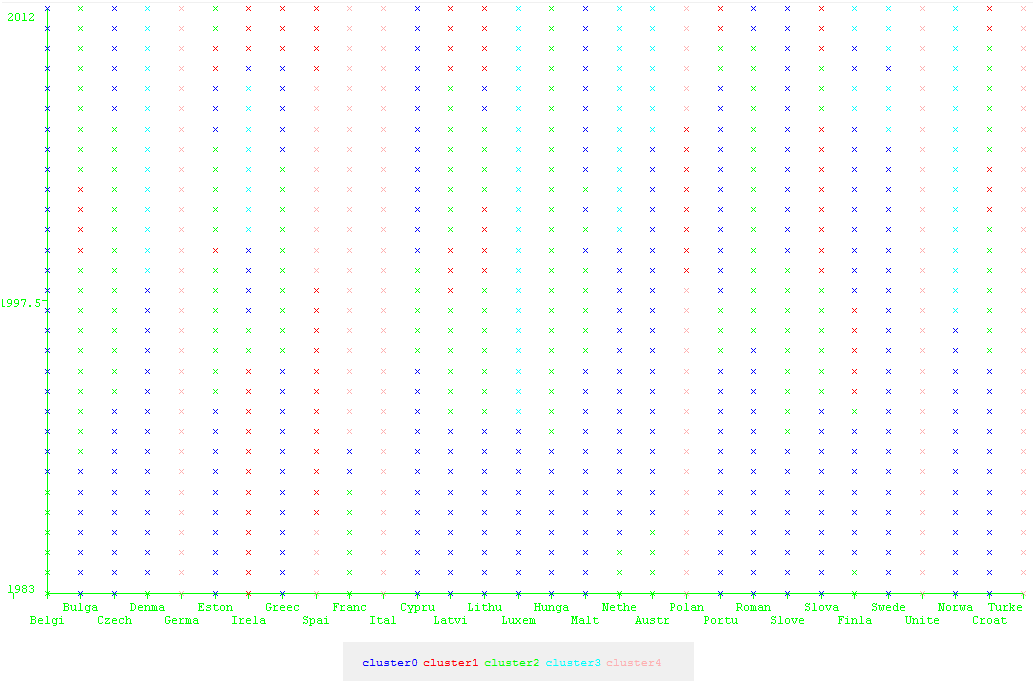
\includegraphics[width=\textwidth]{Appendix/Images/kMeans}
\caption{Graphical representation of what clusters the countries belong to at what year}
\label{fig:clusters}
\end{figure}

From the graph, we can observe that there are three countries that - assuming "often" means seven or more times - change cluster often. They are Estonia, Malta and Finland. Their behaviour is somewhat eratic, however:
\begin{itemize}
	\item Estonia starts in cluster \#0, then changes to cluster \#2 for a long while with one year in cluster \#1. Lastly it moves from cluster \#0 to cluster \#1 to cluster \#2 over the span of a few years.

	\item Malta has a period where it switches between cluster \#0 and \#2 each year over a period of five years, indicating that it is right on the border of the cluster during that period.

	\item Finland moves through all clusters but cluster \#4, though it stays in cluster \#0 for a bit more than half the years.
\end{itemize}

There are also four countries that are the complete opposite, as they never change what cluster they are in. They are Germany, Italy, United Kingdom and Turkey and never leave cluster \#4. Furthermore, they are in the same cluster, which indicates that it is a very stable cluster and they are very stable countries.

Inserting USA into the cluster data (with data from 2011) puts USA in cluster \#4\footnote{See appendix \ref{A_kmr_usa} on \pageref{A_kmr_usa} for the output}. This means that USA is in the same cluster as Germany, France, Italy, United Kingdom and Turkey, which means that USA is more similar to them than any other European country at that time.
\subsection{Frequent Patterns}
\label{Res_FP}

\subsubsection*{Correctness}
\label{Res_FP_Cor}
Even though the association rule has 90\% confidence, it seems unlikely that this rule has any real support. This is due to the fact that it has quite a low support count (1\%) and thus really is not supported by the dataset. Therefore we will disregard it.

If we had lowered our normalisation range to half of what we used, we would most likely have found more occurences of frequent 4-itemsets and generated more association rules. However, lowering the range of our normalisation means differentiating less between the nations and thus making the generated association rules unprecise. Therefore the value of the association rules would be not be very high, as they would not give meaningful insight into how the different values interact.

\section{Conclusion}
\label{Con}
\subsubsection*{The Data}
While we believe that the attributes in the data we use present interesting properties, we should probably have included more attributes to make our results more reliable. If we had included more attributes, we would have been able to discretise more than we have without making all the countries look alike. This would have made it easier to find frequent patterns and made our clustering more precise.
\\We could have used attributes that have little (or nothing) to do with economical qualities of a nation. It would still have been possible to frame similar questions to the ones we present in this project if we had done so.
\subsubsection*{Clustering}
Our clustering results may be skewed by the fact that there is a huge variance in the average of unenmployment rate and population numbers. Without normalisation the Euclidean distance between two population sizes becomes much more significant than the distance between two unemployment rates.

When answering the questions posed in the introduction, we are hesitant to rely on the result of algorithms due to the previosuly mentioned unreliability.
\\If we rely on the results of our mining, the countries that never change cluster are Germany, Italy, Turkey and the United Kingdom. As Germany and the United Kingdom both have had very stable economies over the last three decades, it comes as no surprise to us that they stay within the same cluster for the entire period. Italy has had a mostly stable economy over the last thiry years but was hit very hard by the economic crisis of 2007-current\footnote{http://en.wikipedia.org/wiki/Economy\_of\_Italy\#Late\_2000s\_recession}. Turkey is the result that surprises us the most. Turkey, as a nation, has had quite an unstable economy over the past three decades. While benefitting from the Iran-Iraq war of the 1980s, the Turkish economy was battered in 1991 and plunged into crisis in 1994\footnote{http://en.wikipedia.org/wiki/Economic\_history\_of\_Turkey\#Post\_1950}. With such ups and downs for the Turkish economy, it is highly unlikely that Turkey would stay inside the same cluster when clustering mainly on economic attributes\footnote{We believe it is likely that Turkey staying in the same cluster for the entire period is an example of a skewed result caused by population figures.}. 

There were 1(3) nation(s) that often changed clusters in the period: Finland (and Estonia \& Malta).
\\Finland has an outlier in the period 1992-1996, where it belongs to cluster \#1. This may be an indicator of the fact that the Finnish economy fell into a severe recession in 1991 and then joined the European Union in 1995\footnote{http://en.wikipedia.org/wiki/Economy\_of\_Finland\#Liberalization}.
\\Estonia has been one of the fastest growing economies in the in world in modern times\footnote{http://en.wikipedia.org/wiki/Economy\_of\_Estonia\#The\_economy\_today}. The few years it spends in cluster \#3 may be an indicator of the 2007 financial crisis.
\\Malta has an interesting swing around 2001. Due to the September 11 attacks, the Malta tourist industry suffered a temporary setback - which may be what is reflected here.

It comes as no surprise, to us, that the United States of America is similar to Germany, Italy, Turkey and the United Kingdom considering the possible skewering of results. All three are nations with many inhabitants and relatively stable economies (in 2011).

\subsubsection*{Frequent Patterns}
As we discussed in section \ref{Res_FP}, we found no frequent patterns or association rules with strong support. In the dataset we are working with, a support of exactly 1\% is very weak, and thus the frequent pattern found has very weak support. Therefore we conclude that there are no frequent patterns in the dataset.
\\As we have discussed previously, it is likely that we would be able to find frequent patterns with more support, if we discretised to larger intervals. This would not lead to more reliable results unless more attributes were involved in the mining of a frequent pattern.
\appendix
\settocdepth{chapter}
\chapter{Cluster Images}
\label{APP_CI}
\begin{figure}[!ht]
  \centering
    
\includegraphics[width=\textwidth]{Appendix/Images/Clusters/Temp_Cluster_Image}
  \caption{Cluster Image 1}
  \label{fig:APP_CI_CI1}
\end{figure}
\end{document}